\section{Keeping both branches at finite mass}
\label{sec:twobranch}
We retain the dS$_2$, $L=1$, proper-group, strict-$G_N\to0$ model,
BD vacuum, two equal independent principal-series species, fixed
$\nu,\sigma>0$, and the repeated projections of Section~9. The external
packet is normalized in exact energy. This section separates an identity
for the assembled leading kernel from its error relative to the exact
finite-mass correlator. All proof statements are author self-reviewed
drafts. The two branches originate in KL (B.41)--(B.50)~\cite{KL}; no
new gravitational interaction or priority claim is intended.

\subsection{Conjugate amplitudes with the actual projection}
Put $\ell=\log(2M)$, $T=t-\ell$, and $k=t+\ell=2\ell+T$.
For either protocol let $A_P(\chi)$ denote the integrated minus-branch
amplitude of Section~13, with the density replacements of Section~15
when appropriate. The plus-branch amplitude at the \emph{same}
real $\chi$ is $\overline{A_P(\chi)}$.
This is not the claim $A_Q(-\chi)=\overline{A_Q(\chi)}$, which generally
fails because the projection domain changes with $\chi$.
Indeed the pointwise identity, before any transverse integration, is
\begin{equation}
 \frac{H_\nu V_+}{\pi^3}e^{-\sigma^2\mathcal Q/2}
 =\frac{2^{-2i\chi}\cosh(\pi\chi/2)}{512\pi^7}
 e^{-\sigma^2\chi^2/2}f_{-\chi}(u)f_{-\chi}(v).
 \label{eq:tb-plus-factor}
\end{equation}
For example, the $c$-ratio numerator in $V_+$ contains
$c(1/2+i(x-y\pm\nu))$, and the denominator contains
$c(1/2-i(z\pm\nu))$. They cancel the corresponding oriented external
Gamma factors. The four remaining $x$ factors have common real part
$1/4$ and shift $-i\chi/4$, and likewise for $z$.
Since $f_{-\chi}(w)=\overline{f_\chi(w)}$ for real $\chi,w$, comparison
with (13.3) proves the identity. Multiplication by $\Gamma(i\chi)$
and integration against the same real density and region $D_{r,\chi}$
preserve conjugation.

Define the two-branch leading packet by
\begin{equation}
 X^{(2),P}_M(t)=\operatorname{PV}\int_{\mathbb R}
 \left[e^{iT\chi}A_P(\chi)
       +e^{ik\chi}\overline{A_P(\chi)}\right]\dd\chi.
 \label{eq:tb-definition}
\end{equation}
The two pole residues cancel before integration; for the Gamma and
gapped packets this is an ordinary integral of their combined amplitude.
For other fixed $L^1$ densities use the common approximation prescription
of Section~12. The superscript $(2)$ identifies a leading-kernel
quantity, not an exact 6j evaluation.
\begin{proposition}[Mirror identity]
With $X^P_\infty$ the real fixed-time crossed plateau,
\begin{align}
 X^{(2),P}_M(t)
 &=\mathcal X_P(t-\ell)+\overline{\mathcal X_P(-t-\ell)}-X^P_\infty,
 \label{eq:tb-mirror}\\
 D^{(2),P}_M(t)
 &:=2\bigl(N^P_\infty-\operatorname{Re}X^{(2),P}_M(t)\bigr)\notag\\
 &=\mathcal D_P(t-\ell)+\mathcal D_P(-t-\ell)
                         -\mathcal D_{{\rm edge},P}.
 \label{eq:tb-D}
\end{align}
Here $\mathcal D_{{\rm edge},F}=0$. In particular
$X^{(2),P}_M(-t)=\overline{X^{(2),P}_M(t)}$ and $D^{(2),P}_M$ is even.
\end{proposition}
\begin{proof}
Each Fourier integral in (16.2) is the corresponding $\mathcal X$
minus $X_\infty/2$. Complex conjugation changes the sign of the time
argument. Adding them proves (16.3), and taking real parts proves
(16.4). The same calculation works for every real smooth compact
cutoff before its removal, so also for the regularized definition.
\end{proof}
The fast-branch remainder relative to its delta limit is therefore
$\overline{\mathcal X_P(-k)-X^P_\infty}$, with no fitted time shift.
It retains the full preparation-dependent early tail.

\subsection{A compact estimate that does not differentiate the time phase}
Let $0\le r\le L$ and $|x|,|y|,|z|\le R$, with $L,R$ fixed.
Denote this box by $\Omega_{L,R}$. Set
\begin{equation}
 C^0_M(x,y,z)=\frac{H_\nu(x,y,z)}{\pi^3}
 \left[e^{i\ell\chi}\Gamma(i\chi)V_+
       +e^{-i\ell\chi}\Gamma(-i\chi)V_-\right],
 \quad \chi=x-y+z.
 \label{eq:tb-C0}
\end{equation}
The bracket is evaluated at its removable value when $\chi=0$.
\begin{lemma}[Uniform compact density error]
For $0<\epsilon<1/4$ and sufficiently large $M$, there is a constant
$C_{L,R,\epsilon}$ independent of $M$ and of all real $t$ such that
\begin{align}
 \sup_{\Omega_{L,R}}|\widetilde{\mathcal C}_M-C^0_M|
 &\le C_{L,R,\epsilon}\,e_\epsilon(M),\notag\\
 e_\epsilon(M)&=M^{-1+\epsilon}
       +\frac{1+\ell}{M}+\frac{(1+\ell)^2}{M^2}.
 \label{eq:tb-compact-error}
\end{align}
The same bound times the finite weighted volume controls the truncated
crossed integral, uniformly over all real physical times $t$.
\label{lem:tb-compact}
\end{lemma}
\begin{proof}
Use $\Lambda=M$ in Theorem~11.1. On the box,
\[
 s(M+\xi)-M=\xi-\frac{1}{8M}+O_{L,R}(M^{-2}),
 \qquad j(M+\xi)=1+O_{L,R}(M^{-2}).
\]
The common $-1/(8M)$ cancels in every label difference. The external
factor divided by $M$ differs from $H_\nu$ by $O_{L,R}(M^{-1})$.
The assembled bracket is $O_{L,R}(1+\ell)$ and its first offset
derivatives are $O_{L,R}((1+\ell)^2)$. To see this through $\chi=0$,
subtract its explicit sinc term (11.11); its smooth remaining
amplitudes multiply $e^{\pm i\ell\chi}$. Differentiating the sinc
costs at most $O(\ell^2)$. This controls the $O(M^{-2})$ change of
differences without differentiating the unknown exact remainder.
Multiplication by the external factor and the three Jacobians gives
(16.6). Crucially, both densities are compared in the \emph{same exact
energy coordinates}, then multiplied by the identical unit-modulus
factor $e^{it\chi}$. There is no $|t|$ loss in this comparison.
Bounded hard indicators can be retained in its ordinary compact integral.
\end{proof}
This improves the deliberately coarse phase-change argument in
Section~12. It does not supply bounds on $C_{L,R,\epsilon}$ as the box
grows with $M$.

\subsection{Uniform absolute approximation on the full time axis}
Let $A,B,b$ be the positive-envelope quantities in Section~9 and put
\begin{align}
 \tau_X(L,R)&=2A\sqrt{2A b(R/2)}
                  +A^2\int_L^\infty\pi_0(r)\dd r,\notag\\
 \tau_N(L,R)&=2A b(R/2)+A^2\int_L^\infty\pi_0(r)\dd r.
 \label{eq:tb-tails}
\end{align}
The external tail is a Gamma survival function or a shifted exponential
for the packets of Section~15, and $b$ is a Gaussian tail. Their
constants remain those of the analytic envelope, not certified numbers.
\begin{theorem}[Two-branch absolute approximation]
For either fixed protocol and every fixed normalized $L^1$ external
density, with fixed $\nu,\sigma>0$,
\begin{equation}
 \sup_{t\in\mathbb R}|X^P_M(t,0,t,0)-X^{(2),P}_M(t)|\longrightarrow0.
 \label{eq:tb-uniform-X}
\end{equation}
More precisely, for each fixed box and sufficiently large $M$,
\begin{align}
 \sup_t|X^P_M-X^{(2),P}_M|
 &\le C_{L,R,\epsilon}'e_\epsilon(M)+4\tau_X(L,R),\notag\\
 |N^P_M-N^P_\infty|
 &\le C''_{L,R}/M+2\tau_N(L,R).
 \label{eq:tb-cutoff-bound}
\end{align}
Consequently $\delta_M^P:=\sup_t|D^P_M(t)-D^{(2),P}_M(t)|\to0$.
No explicit rate for this supremum is claimed.
\label{thm:tb-uniform}
\end{theorem}
\begin{proof}
Truncate each ordered tree as in Proposition~9.1 and discard $r>L$.
The exact crossed error is at most $\tau_X$, uniformly in $M,t$.
The truncated two-branch expression satisfies the same mirror identity,
with truncated limiting curves $\mathcal X_{L,R}$ and plateau
$X_{\infty,L,R}$. These curves can first be defined with smooth cutoffs
and thresholds; the norm bounds allow their removal. Equivalently,
on this compact box the transverse integral has a locally Lipschitz
amplitude at $\chi=0$: moving any of the finitely many linear faces
changes a volume by $O(|\Delta\chi|)$, uniformly in bounded $r$, and
the remaining smooth integrand has bounded derivatives. Integration
against the $L^1$ density preserves this bound. Its pole-subtracted
PV thus exists, including the hard faces.

For each fixed argument $U$, take the logarithmic-time limit of the
exact full and truncated pairings. Their difference is at most
$\tau_X$, so $|\mathcal X_P(U)-\mathcal X_{L,R}(U)|\le\tau_X$
for \emph{every} real $U$. This gives a supremum bound without
interchanging a supremum and a convergence limit. The fixed-time limit
likewise gives $|X^P_\infty-X_{\infty,L,R}|\le\tau_X$.
The mirror identity now bounds the full-minus-truncated two-branch
expression by $3\tau_X$, independently of $M,t$. On the compact box
Lemma~\ref{lem:tb-compact} bounds the remaining exact-minus-leading
difference. This proves the first inequality in (16.9).

The positive ordered norms have excluded mass at most $\tau_N$.
Their compact one-step Gamma-ratio error is $O_{L,R}(M^{-1})$;
passing the same tail bound to the limit proves the second inequality.
For the fixed threshold the boundary has left the box once $M$ is
large enough. The moving threshold is identical in both integrands.
Finally, first choose $L,R$ large at fixed parameters, then take $M$
large. The commutator error is at most twice the crossed error plus
twice the norm error, proving the assertion.
\end{proof}
This theorem keeps both branches. Replacing the second branch by its
delta before applying the theorem would give a different approximation
and would discard the correction examined next.

\subsection{Which early signals can the fast branch compete with?}
Write $t=\ell-s$ so that $T=-s$ and $k=2\ell-s$. Assume $s,k\to\infty$.
Let $E_P(s)=\mathcal D_P(-s)-\mathcal D_{{\rm edge},P}$. Exactly,
\begin{equation}
 D^{(2),P}_M(\ell-s)-\mathcal D_{{\rm edge},P}=E_P(s)+E_P(k).
 \label{eq:tb-early-sum}
\end{equation}
For a Gamma packet with nonzero real coefficient $c_p$ in \eqref{eq:dep-real-tail}, put
$n=p+3$ for even $p$ and $n=p+4$ for odd $p$. Then
\begin{align}
 D^{(2),p}_M(\ell-s)-\mathcal D_{{\rm edge},p}
 &=c_p(s^{-n}+k^{-n})+O(s^{-n-1}+k^{-n-1}),\notag\\
 \frac{E_p(k)}{E_p(s)}
 &=\left(\frac{s}{k}\right)^n[1+O(s^{-1}+k^{-1})].
 \label{eq:tb-power-window}
\end{align}
In particular, for $s=a\ell$ with fixed $0<a<2$, the relative
fast-branch contribution tends to $(a/(2-a))^n$, not zero.
For positive physical times in this scaling take $0<a<1$.
Dropping the fast branch is relatively valid for these power tails
only when $s/k\to0$, equivalently $s=o(\ell)$ in the early regime.
The critical odd-$p$ density with $c_p=0$ is excluded.
At fixed $T$, the fast residual itself has a power of $\log M$;
this is a statement about the two-branch expression, not a determined
leading rate for the exact-minus-single-branch correlator.

For the fixed-threshold Gaussian, (13.6) instead gives, for $2<h<4$,
\begin{equation}
 D^{(2),F}_M(\ell-s)
 =2C_{\nu,\sigma}(e^{-2s}+e^{-2k})
      +O(e^{-hs}+e^{-hk}).
 \label{eq:tb-exponential-window}
\end{equation}
Its fast/slow ratio is $e^{-4t}[1+o(1)]$, so relative suppression
requires $t\to+\infty$ while $s\to\infty$. For a fixed gap,
\begin{equation}
 D^{(2),g}_M(\ell-s)-\mathcal D_{{\rm edge},g}
 =-2\operatorname{Re}\left[C_g\left(\frac{e^{igs}}{s^4}
                          +\frac{e^{igk}}{k^4}\right)\right]
    +O(s^{-5}+k^{-5}).
 \label{eq:tb-gap-window}
\end{equation}
Near zeros of the first oscillatory term only an envelope comparison
is meaningful; there is no uniform relative estimate there.

To transfer any displayed small signal to the exact finite-$M$
observable one must additionally have $\delta_M^P=o(s^{-n})$,
$o(e^{-2s})$, or $o(s^{-4})$, respectively. Theorem~16.3 proves
$\delta_M^P\to0$, not these explicit rates. It does imply existence
of some slowly growing windows. For a noncritical Gamma packet one
may take, for sufficiently large $M$,
\[
 s(M)=\min\{\sqrt\ell,(\delta_M^P)^{-1/(2n)}\},
\]
with the second entry interpreted as infinity at zero error. Then
$s\to\infty$, $s=o(\ell)$ and $\delta_M^P s^n\to0$.
For $F$ replace the second entry by
$\tfrac14\log(1/\delta_M^F)$, which gives
$\delta_M^F e^{2s}\to0$. These are existence constructions in terms
of an unknown error, not computable experimental windows. Quantifying
the growth of the compact constants in (16.9) is still required.

\subsection{Checks and the remaining finite-mass task}
The accompanying calculation verifies (16.1) directly from the original
$c$ ratios at high precision. It then reuses the frozen full projected
spectra of Sections~14--15, combines the two amplitudes before quadrature,
and compares with (16.3). Small early differences are formed from the
pole-subtracted integrals, not by subtracting two plateau-sized values.
The numerical records distinguish exact algebra, empirical quadrature,
and the still-uncomputed exact finite-mass remainder.

At $\nu=0.6$, $\sigma=\beta=1$, 300 empirical diagnostics pass.
For $s=\ell/2$ and $\ell=40$, the directly integrated fast/slow
real-correction ratios for $p=0,1,2$ are respectively $0.043283$,
$0.005156$, and $0.005305$. Their asymptotic targets are $1/27$,
$1/243$, and $1/243$. The three independent stored quadrature rules
give maximum relative changes of the small real quantities of
$4.14\times10^{-8}$, $4.30\times10^{-4}$, and $6.69\times10^{-4}$,
respectively; the gapped case gives $3.60\times10^{-6}$.
These are empirical refinement differences, not certified total errors.
The $p=2$ slow correction has not reached its negative asymptotic
regime at $\ell=16$; its negative fast/slow ratio there is retained
in the data. Figure~\ref{fig:tb-window} shows only $\ell\ge24$ to
resolve the subsequent approach, without treating earlier sign changes
as numerical failures.
\begin{figure}[htbp]
 \centering
 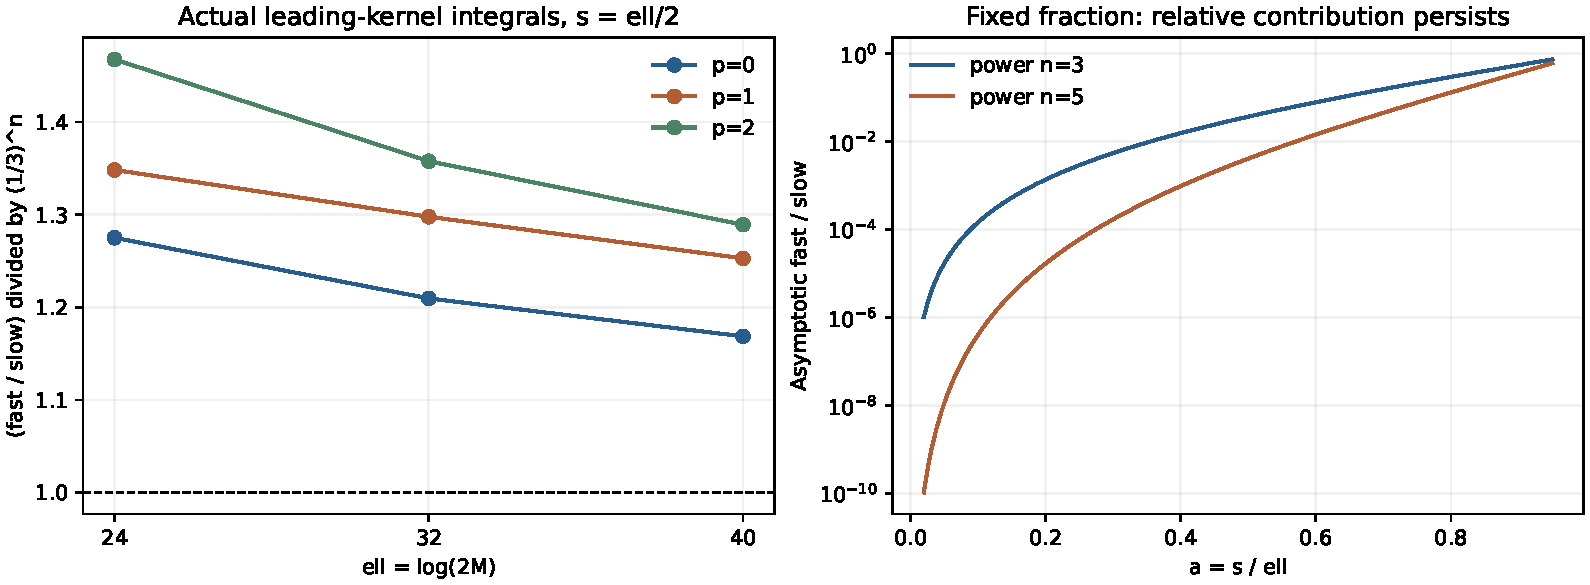
\includegraphics[width=.98\linewidth]{../results/stage3/two-branch/branch-window.pdf}
 \caption{Left: actual two-branch leading-kernel packet integrals, with
 $s=\ell/2$ and $k=3\ell/2$, normalized by the asymptotic fast/slow
 ratio. Right: the analytic limiting ratio for fixed $a=s/\ell$.
 Neither panel is an exact finite-$M$ 6j calculation.}
 \label{fig:tb-window}
\end{figure}

The next task is to bound $C_{L,R,\epsilon}'$ and $C''_{L,R}$ for an
explicit growing choice of $L,R$. Gaussian path tails suggest
$R$ of order $\sqrt{\log\log M}$ and exponential external tails suggest
$L$ of order $\log\log M$ for inverse-logarithmic target errors, but
these choices are not justified until the local constants are tracked.
No threshold smoothing loss is necessary for the compact two-branch
comparison; the positive-tail argument controls its removal globally.
Exact 6j packet calculations and total certified numerical errors remain
separate open work, as do finite-$G_N$ dynamics and a complete dual.
